\normalfont\normalsize
\chapter{Energy Harvesting}

This chapter presents the energy harvesting platform.

It is difficult to chose the best solution for solar energy harvesting, due to power requirements
of different applications. In this chapter we will present the hardware that we used to generate
and store solar energy.

\begin{figure}[ht] \centering
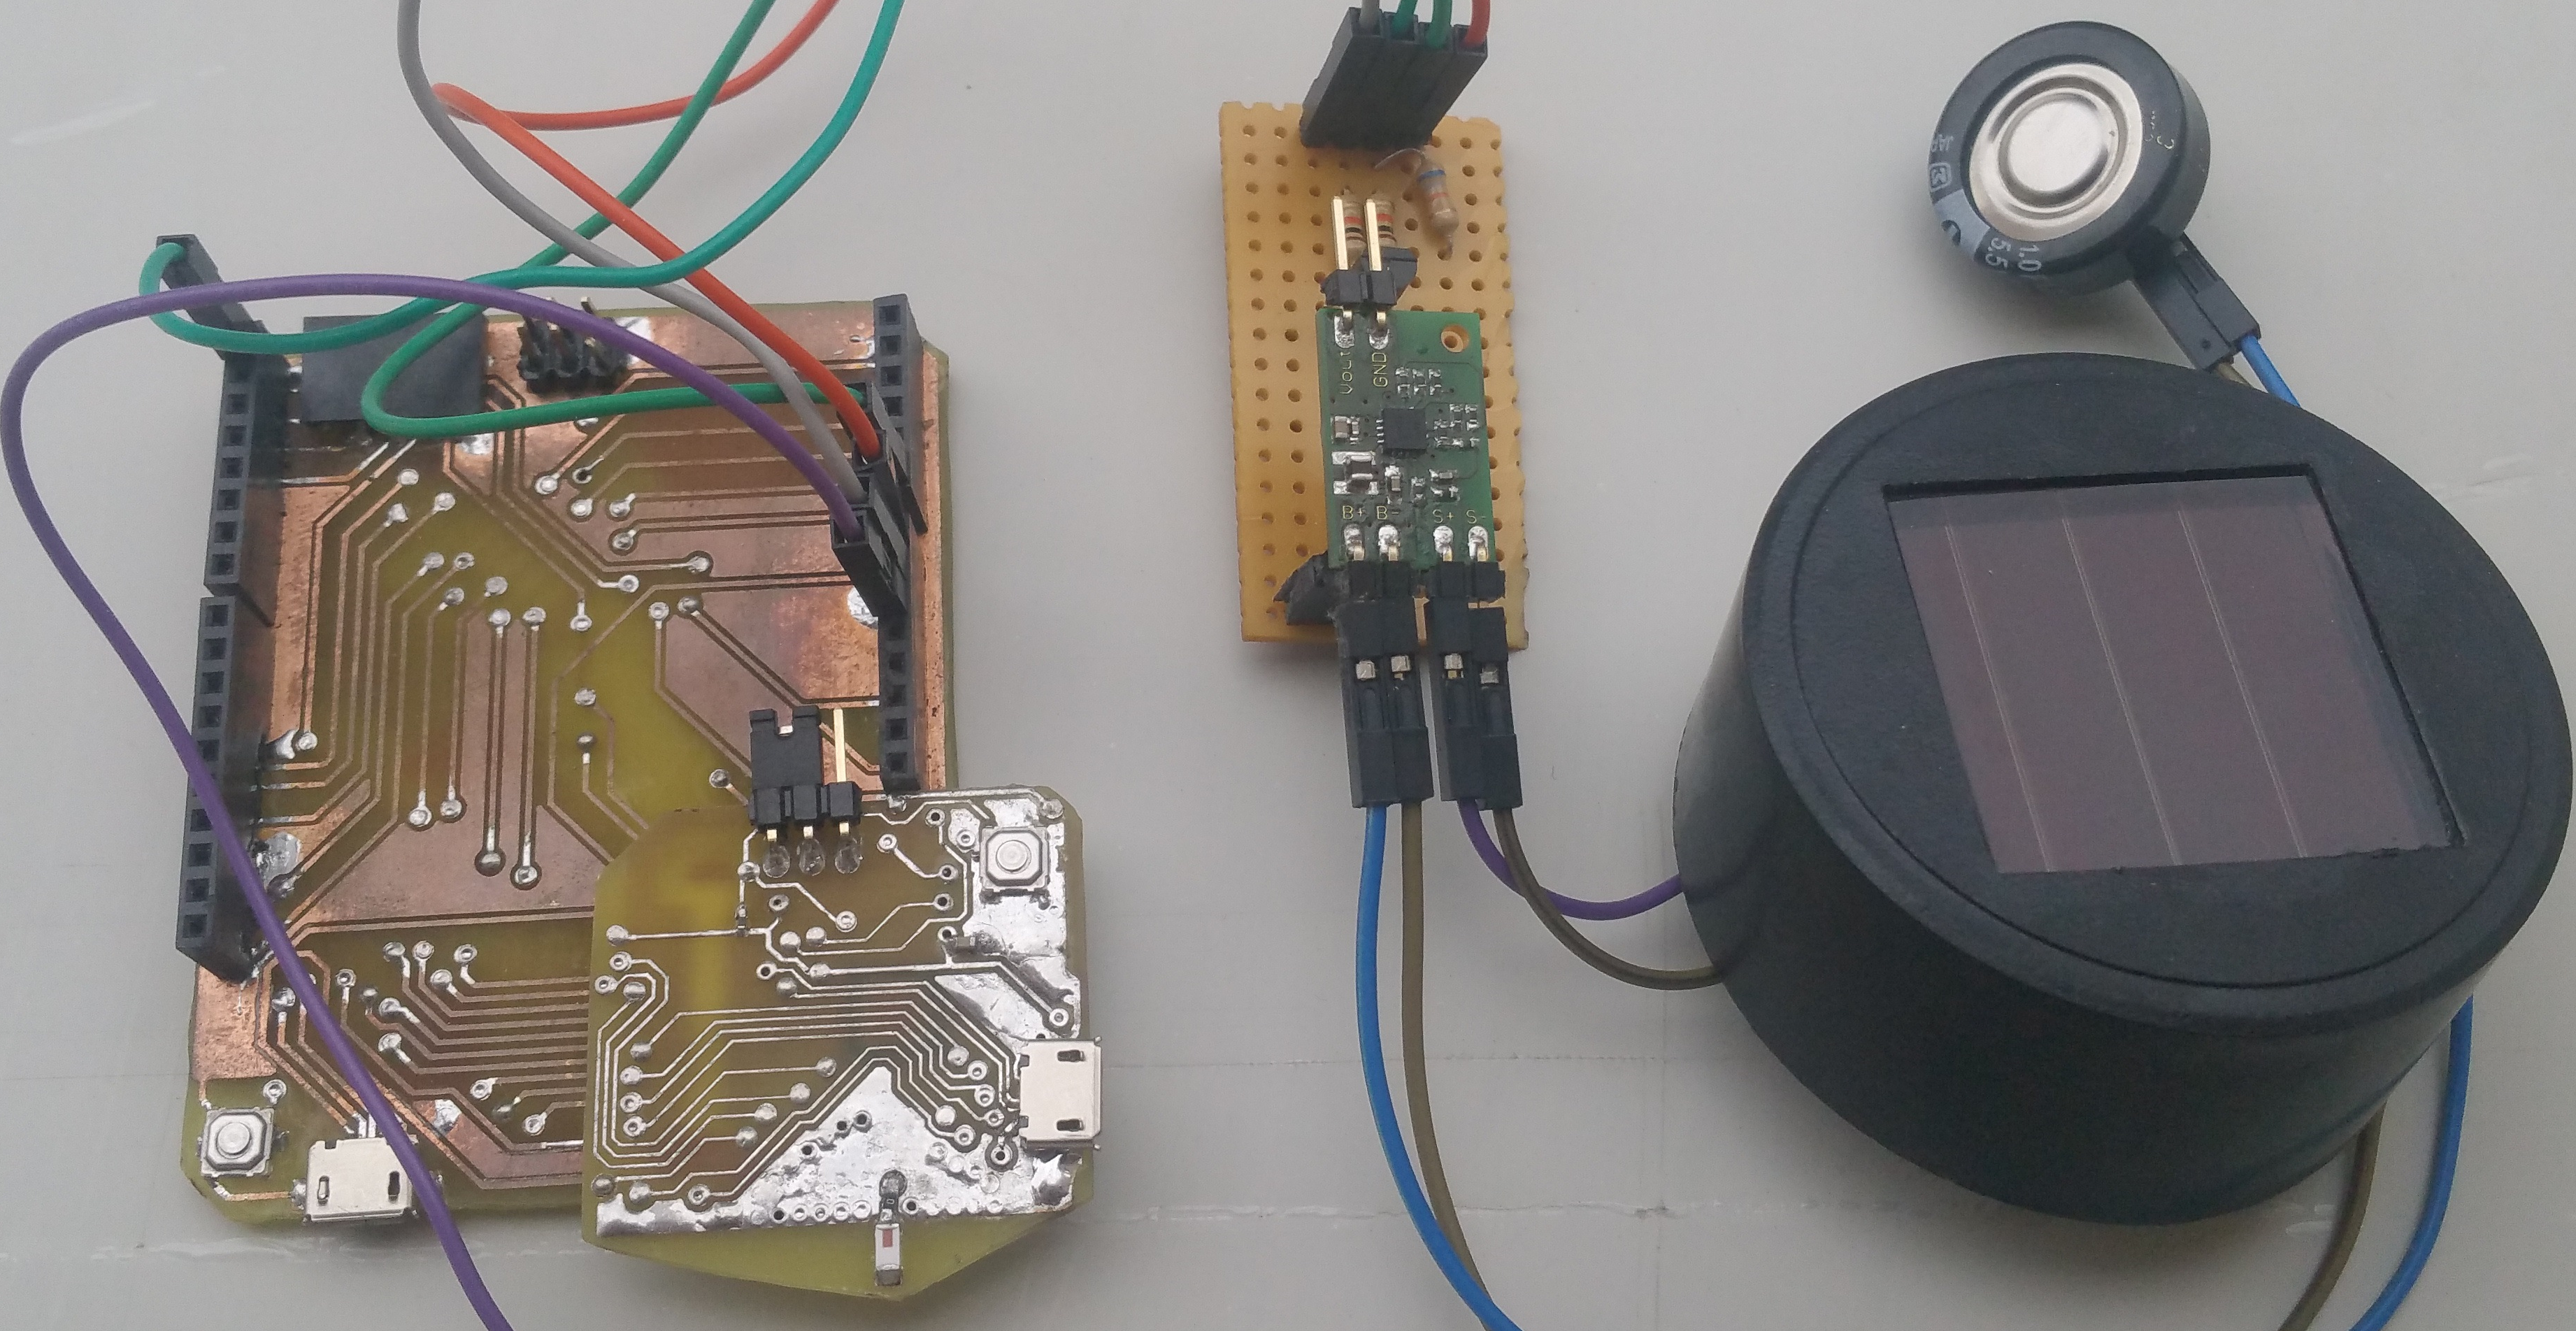
\includegraphics[width=0.85\textwidth]{img/ehvsetup.png}
\caption{Setup for solar energy harvesting}
\end{figure}

\section{TI BQ25504}
The main component of an energy harvester is the boost converter needed to raise the voltage of the
solar cell in order to be able to charge a battery or a super-capacitor. The chip selected by us is
TI BQ25504, a very efficient boost converter with battery management for energy harvesting.

The chip can begin charging from a low voltage of only 330mV, has a very small quiescent current,
less then 360nA and once started, it can harvest energy until the voltage drops down to 80mV.

Another advantage is that the output voltage can be selected from 2.5V up to 5.25V, which can be
used, as demonstrated in previous chapter, to charge a capacitor to a higher voltage in order
to exponentially increase the total amount of stored energy.

Four our experiment, we have selected an output voltage of 3300mV.

\section{Super-capacitor}
The advantages of the super-capacitor over the rechargeable battery are as follows:

\begin{itemize}
\item it can charge and discharge almost instantaneously
\item it has a very high number of charge/discharge cycles
\item it does not suffer from the same aging symptoms as a battery
\item it more eco-friendly than a standard battery
\item it will allow a longer maintenance-free time than a battery

\end{itemize}

The disadvantages of the super-capacitor are :

\begin{itemize}
\item it is bigger than a similar capacity battery
\item it can store a much smaller amount of energy than similar sized batteries
\item it is very expensive
\item it operates at low voltages and may require a charge pump to raise the voltage
\item higher current leakage.

\end{itemize}

The main problem of a capacitor is current leakage. The bigger the capacitor, the bigger the
current leakage. Also the technology with which they are built, the number of cycles or age can
also have a profound effect on leakage current.

Even though it does not seem much, if a 1F capacitor has self discharge rate of 6uA
\cite{ultracap}, this is more than the sleep power of the Sparrow R. Even more, if using a 25F
capacitor, the leakage current is increased to 45uA, which can be equivalent to the same power
consumption of the node sending data every few seconds. Because of this, the total energy that can
be stored is greatly affected by the duration needed for the node to use the super-capacitor as
power supply.

Charging is also a problem. If for 1F capacitor, a panel that can supply 50uA is more than enough to charge
the capacitor and supply power to the node, for a 25F capacitor that power is barely enough
to maintain the stored energy, without even powering the node.

For our experiments we have chosen two 1F capacitors rated at 5V.

\section{Solar Panel}

We can use any solar panel, as long as it is rated up to 3V and has enough power to charge the
selected capacitor.

Because we do not need a large amount of energy, a small solar cell of just 60mW is more than
enough to fully charge the capacitor in just 5 minutes of sunny weather. This means that regardless
of the meteorological condition, we would be able to charge the capacitor daily.

